\documentclass[11pt]{article}

\usepackage{fullpage}
\usepackage{caption}
\usepackage{float}

\usepackage[T1]{fontenc}
\usepackage{textcomp}

\usepackage[english]{babel}
\usepackage[utf8]{inputenc}

\usepackage{lmodern}

\usepackage{hyperref}
\hypersetup{breaklinks}
\hypersetup{pdfborder=0 0 0}

\usepackage[babel=true]{microtype}


\usepackage{amsmath}
\renewcommand{\vec}[1]{\mathbf{#1}}
\newcommand{\mat}[1]{\mathbf{#1}}
\DeclareMathOperator{\Prob}{Prob}
\newcommand{\md}{\mathrm{d}}
\newcommand{\me}{\mathrm{e}}
\newcommand{\mT}{\mathrm{T}}

\usepackage{units}
\usepackage{tikz}
\usepackage[square,sort,comma,numbers]{natbib}
\usepackage{hypernat}

\allowdisplaybreaks[1]

\title{Supporting Information: \\
\textbf{Interactions between chronic diseases: 
asymmetric outcomes of co-infection at individual and population scales}}
\date{}
\author{Erin E. Gorsich$^{a,b*}$, Rampal S. Etienne$^{c}$, Jan Medlock$^{a}$, \\ Brianna R. Beechler$^{a}$, Johannie M. Spaan$^{b}$, Robert S. Spaan$^{d}$, \\Vanessa O. Ezenwa$^{e}$, Anna E. Jolles$^{a,b}$}

\begin{document}

\maketitle

\noindent{}a. Department of Biomedical Sciences, 105 Dryden Hall, Oregon State University \\
\noindent{}b. Department of Integrative Biology, Cordley Hall, Oregon State University \\
\noindent{}c. Groningen Institute for Evolutionary Life Sciences, University of Groningen, The Netherlands\\
\noindent{}d. Department of Fisheries and Wildlife, 104 Nash Hall, Oregon State University \\
\noindent{}e. Odum School of Ecology and Department of Infectious Diseases, College of Veterinary Medicine, University of Georgia \\
\noindent{}$ \ast$ Corresponding author e-mail: eringorsich@gmail.com \\



\noindent \Large{\textbf{Appendix 3. Additional information on field methods and diagnostic testing}}\\
%\normalize

Detailed capture information, including chemical immobilization methods and recapture rates have been described previously \cite{beechler_enemies_2015, gorsich_context-dependent_2015, ezenwa_opposite_2015}. We collected all field data Kruger National Park (KNP), South Africa. Data collection methods for the results presented in this work are summarized briefly here. 

\subsection*{Buffalo cohort study}
 We conducted a longitudinal study of 151 female buffalo to estimate the consequences of BTB and brucellosis infection. An initial 104 female buffalo were captured between June 2008 and October 2008. Buffalo were captured at two locations in the southeastern section of KNP. Fifty-three buffalo were captured in the Lower Sabie region; fifty-one were captured in the Crocodile Bridge region (Fig S8). Buffalo were radio-collared for re-identification and captured biannually at approximately 6 month intervals from their initial capture in 2008 until August of 2012. As natural mortalities occurred throughout the study period, new buffalo were captured and monitored, so that 47 buffalo were added throughout the course of the study.
 
During each capture, we recorded brucellosis infection status, BTB infection status, age, and the animals' reproductive status. Buffalo age was assessed by tooth eruption in younger buffalo and by incisor wear in older buffalo \cite{jolles_population_2007}. Reproductive status was quantified by whether the buffalo had a calf (defined as animals < 1 year old) at the capture immediately following the birthing season (March - July; \cite{gorsich_context-dependent_2015}). For each capture, we used a combination of visual siting and lactation status to identify buffalo with calves. Buffalo calves often associate with their mother until the next breeding season and were distinguishable from other calves by being within a few meters from the female. In 6\% (13/ 204) of observations, calf status was marked as unknown when a calf was observed but it was not clear who was the mother. In these cases, the focal animal was identified as having a calf only if they were lactating. \\

\subsection*{Disease testing}
Blood was collected by jugular venipuncture into lithium heparinized tubes for BTB diagnostics and into tubes with no additives for brucellosis diagnostics. Diagnosis of brucellosis was based an ELISA test (Brucellosis Serum Ab ELISA test, IDEXX). The brucellosis ELISA detects the presence of antibodies in serum and has an estimated sensitivity of 93\% and specificity of 87\% in African buffalo \cite{gorsich_evaluation_2015}. Diagnosis of BTB infection was determined based on a whole blood gamma interferon ELISA assay (BOVIGAM ELISA kit, Prionics; \cite{michel_approaches_2011}). The BOVIGAM assay for BTB identifies an infected animal based on the \textit{in vitro} production of IFN-gamma by whole blood after stimulation with \textit{Mycobacterium bovis} antigen (bovine tuberculin). Diagnosis of BTB is complicated by non-specific reactivity to environmental mycobacteria, including \textit{Mycobacterium avium} antigens. Therefore, we followed an established protocol that accounts for exposure to \textit{M. avium} because it has an estimated sensitivity of 86\% and specificity of 92\% after optimization for use in African buffalo \cite{michel_approaches_2011}. For a few captures, diagnosis was not possible if blood collection was incomplete or if errors in testing resulted in unclear test results. Removal of these capture events resulted in the removal of only six buffalo from our dataset (146 buffalo sampled).

\begin{figure}[H]
\centering
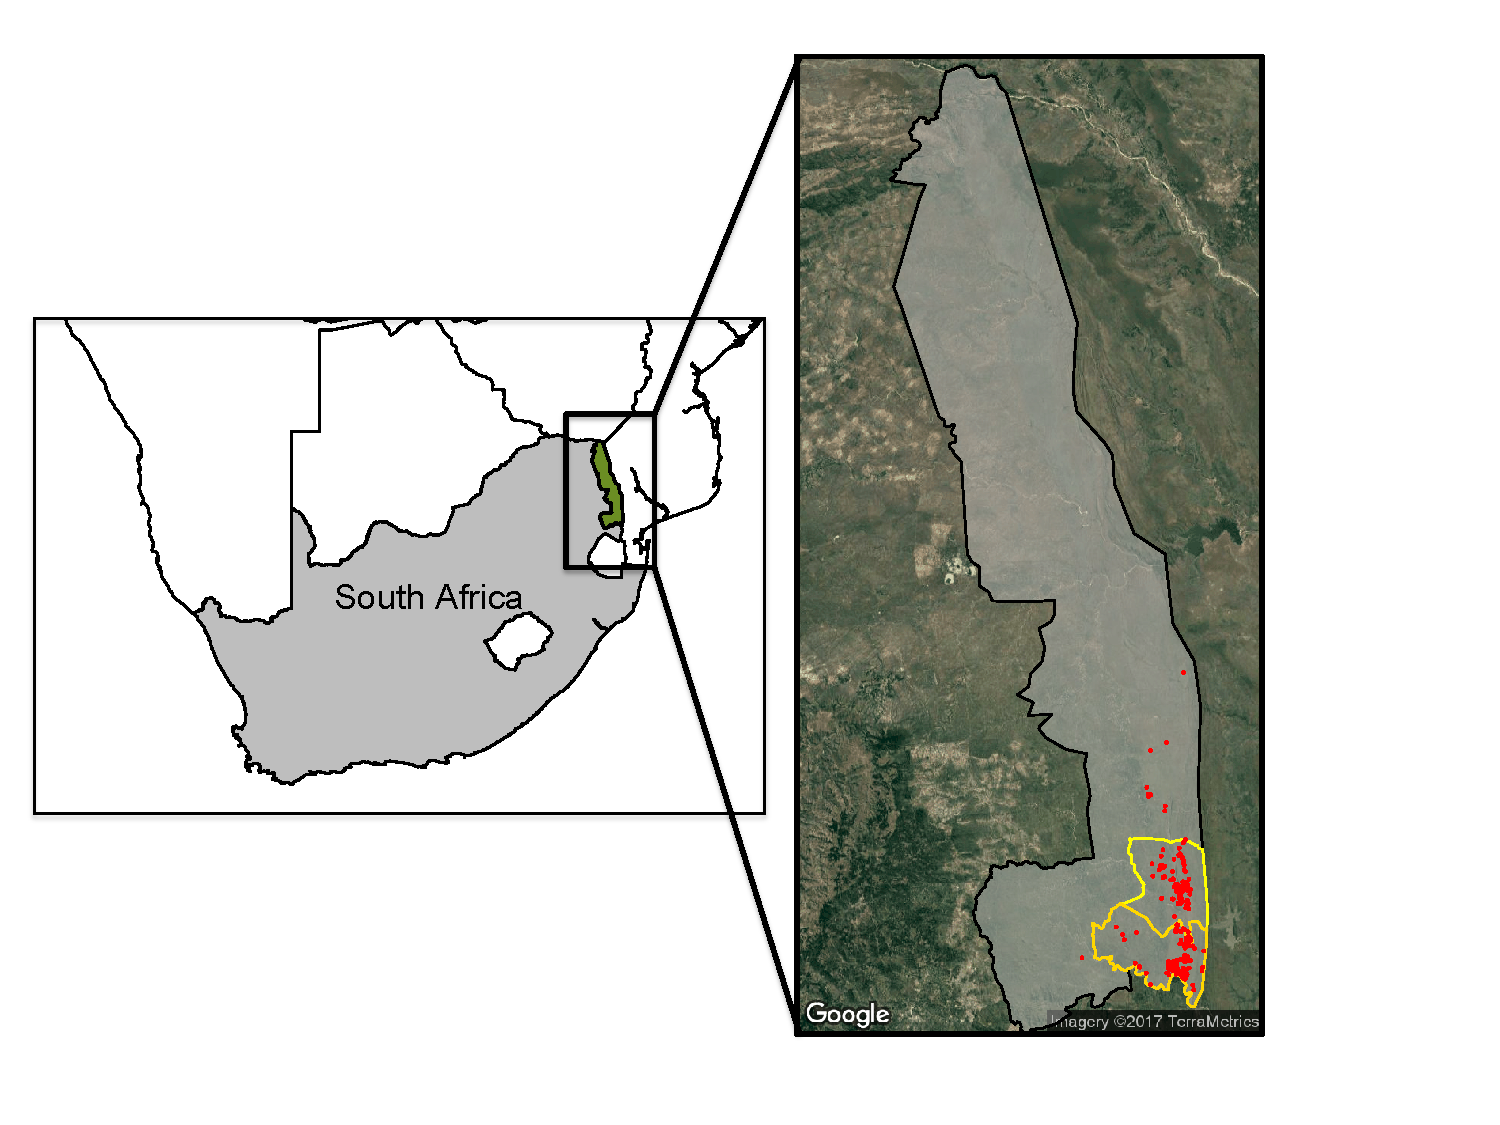
\includegraphics[width=.99\linewidth]{Figure_S8.pdf}
\caption*{\textbf{Fig S8.} Kruger National Park is on the northeastern boundary of South Africa.  The blown-up figure shows a google maps image of the park. Buffalo were initially captured in the Lower Sabie (light yellow) Crocodile Bridge sections (dark yellow) of the park. Red dots represent the re-capture locations for the subsequent capture. We account for initial capture location in all statistical analyses although more detailed analyses of how buffalo move over time and space are underway.}
\end{figure}

\pagebreak

\bibliographystyle{pnas-new}
\bibliography{coinfection}




\end{document}